\documentclass[aspectratio=169]{beamer}
\usepackage{will_handley_beamer}
\usepackage{title_page}

% Commands
% --------
% - \arxiv{arxiv number}
% - \arxiv{<number>}            arxiv.org/abs/<number>
% - \oldarxiv{<arxiv number>}   arxiv.org/<number>
% - \doi{<doi>}                 doi.org/<doi>
% - \xkcd{<number>}             xkcd.com/<number>
% - \email{<email>}             <<email>>
% - \tthref{<website>}          <website>
% - \av[dist]{<quantity>}       <quantity>_{dist}
% - \student{<name>}{<detail>}{<photo>}

% A simple command for highlighting key terms
\newcommand{\keyterm}[1]{\textbf{\textcolor{C0}{#1}}}

% Talk details
% ------------
\title{A Statistician's Guide to the Galaxy (Fitting Zoo)}
\subtitle{An Introduction to the Statistical Foundations of SED Fitting}
\date{8 July 2025}

\begin{document}

% --- SLIDE 0: Title Slide ---
\begin{frame}
    \titlepage
\end{frame}

% --- SLIDE 1: SED Fitting Setup (2 minutes) ---
\begin{frame}
    \frametitle{The Goal: From Photons to Physics}
    \framesubtitle{Why SED fitting is a statistical inference problem}
    \begin{columns}[T]
        \column{0.49\textwidth}
        \begin{block}{The Data $D$}
            We observe a galaxy's light (photometry or spectra) across different wavelengths. This is our dataset, $D$.
        \end{block}
        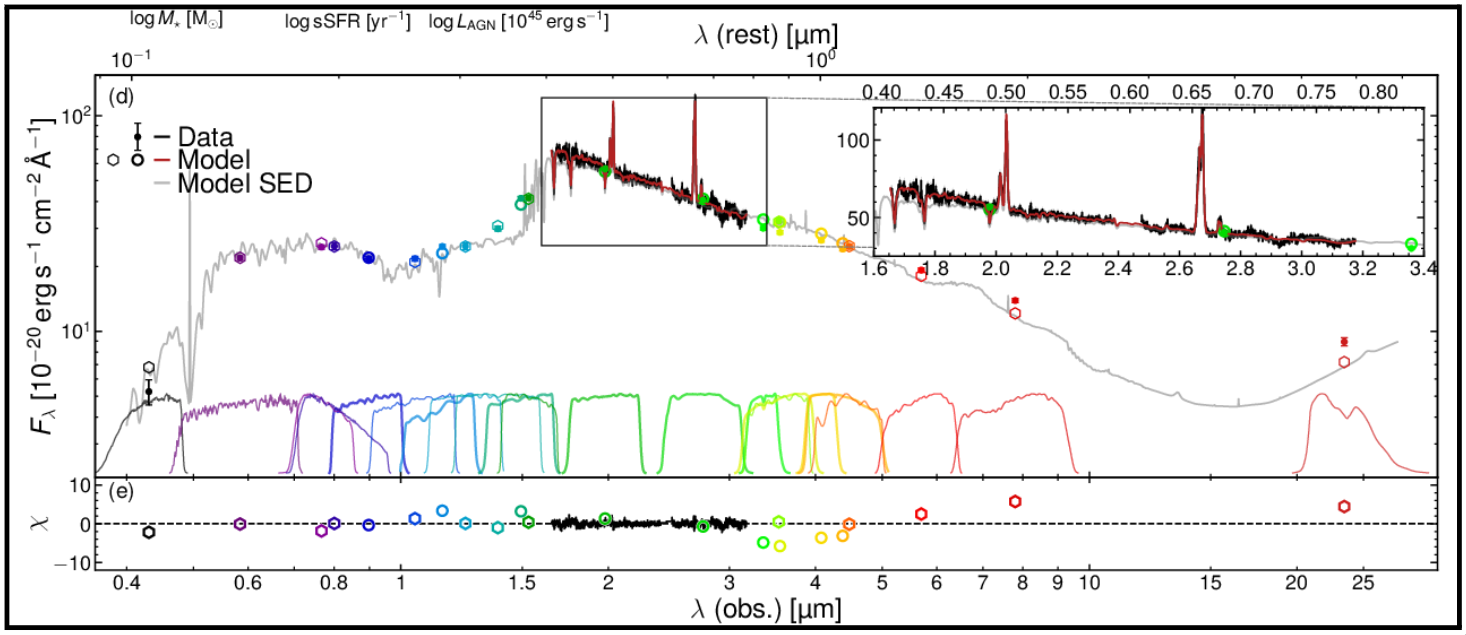
\includegraphics[width=\textwidth]{figures/sed.png}
        \column{0.49\textwidth}
        \begin{block}{The Model $\theta|M$}
            We want to infer the underlying physical properties, our parameters, $\theta$: Stellar Mass ($M_*$), Star Formation History (SFH), Dust content ($A_V$), Metallicity ($Z$), ...
        \end{block}
        \begin{block}{The Challenge}
            The parameter space is often:
            \begin{itemize}
                \item \keyterm{High-dimensional}: Many parameters to fit.
                \item \keyterm{Degenerate}: Different combinations of parameters can produce similar SEDs.
            \end{itemize}
        \end{block}
    \end{columns}
\end{frame}

% --- SLIDE 2: Statistical Framework (2 minutes) ---
\begin{frame}
    \frametitle{The Language of Inference: }
    \framesubtitle{How we quantify what we learn from data}
    \begin{columns}
        \column{0.33\textwidth}
            \begin{block}{\C[1]{Prior}\hfill $\C[1]{\pi(\theta)}$}
                What we believe about the parameters \textit{before} we see the data. Our physical assumptions.
            \end{block}
        \vspace{2em}
        \begin{block}{\C[3]{Evidence}\hfill $\C[3]{\mathcal{Z}(D)}$}
            How we update our belief in the model using the data.
        \end{block}
        \column{0.33\textwidth}
\[\underbrace{\C[0]{\mathcal{P}(\theta|D)}}_{\C[0]{\text{Posterior}}} = \frac{\overbrace{\C[2]{\mathcal{L}(D|\theta)}}^{\C[2]{\text{Likelihood}}} \times \overbrace{\C[1]{\pi(\theta)}}^{\C[1]{\text{Prior}}}}{\underbrace{\C[3]{\mathcal{Z}(D)}}_{\C[3]{\text{Evidence}}}}\]
        \column{0.33\textwidth}
            \begin{block}{\C[2]{Likelihood}\hfill $\C[2]{\mathcal{L}(D|\theta)}$}
                How we update our belief in the parameters using the data.
            \end{block}
        \vspace{2em}
        \begin{block}{\C[0]{Posterior}\hfill $\C[0]{\mathcal{P}(\theta|D)}$}
            What we know about the parameters \textit{after} seeing the data. It's our updated state of knowledge.
        \end{block}
    \end{columns}
\end{frame}

% --- SLIDE 3: Chi-squared Maximization (3 minutes) ---
\begin{frame}<1-10>
    \frametitle{The Simplest Approach: Optimization (e.g., $\chi^2$ Minimization)}
    \begin{columns}[T]
        \column{0.5\textwidth}
        \only<1-6>{
        \begin{block}{How it Works: Hill Climbing}
            Imagine the parameter space is a landscape where lower $\chi^2$ (or higher likelihood) is ``downhill''.
            \begin{itemize}
                \item Start somewhere.
                \item Follow the steepest gradient downhill.
                \item Stop when you reach the bottom of a valley.
            \end{itemize}
        \end{block}
        \begin{block}{Advantages}
            \begin{itemize}
                \item \keyterm{Fast} and computationally cheap.
                \item Good for a quick first look.
            \end{itemize}
        \end{block}
        }
        \only<7-10>{
        \begin{block}{Limitations}
            \begin{itemize}
                \item Only gives a single \keyterm{point estimate} (the ``best fit'').
                \item \textbf{No uncertainty quantification!} Where are the error bars?
                \item Can easily get stuck in a \keyterm{local minimum}, missing the true global best fit.
            \end{itemize}
        \end{block}
        \begin{alertblock}{Key Message}
            Optimization is fast but gives an incomplete and potentially misleading picture. Science needs error bars.
        \end{alertblock}
        }
        \column{0.5\textwidth}
        \vspace{-1.8em}
        \begin{center}
            \includegraphics<1>[width=\textwidth,page=1]{figures/himmelblau_gradient_ascent.pdf}%
            \includegraphics<2>[width=\textwidth,page=2]{figures/himmelblau_gradient_ascent.pdf}%
            \includegraphics<3>[width=\textwidth,page=3]{figures/himmelblau_gradient_ascent.pdf}%
            \includegraphics<4>[width=\textwidth,page=4]{figures/himmelblau_gradient_ascent.pdf}%
            \includegraphics<5>[width=\textwidth,page=5]{figures/himmelblau_gradient_ascent.pdf}%
            \includegraphics<6>[width=\textwidth,page=6]{figures/himmelblau_gradient_ascent.pdf}%
            \includegraphics<7>[width=\textwidth,page=7]{figures/himmelblau_gradient_ascent.pdf}%
            \includegraphics<8>[width=\textwidth,page=8]{figures/himmelblau_gradient_ascent.pdf}%
            \includegraphics<9>[width=\textwidth,page=9]{figures/himmelblau_gradient_ascent.pdf}%
            \includegraphics<10>[width=\textwidth,page=10]{figures/himmelblau_gradient_ascent.pdf}%
        \end{center}
    \end{columns}
    
\end{frame}

% --- SLIDE 4: Why do sampling? (3 minutes) ---
\begin{frame}
    \frametitle{Why do sampling?}
    \begin{columns}[T]
        \column{0.5\textwidth}
        \begin{itemize}
            \item The cornerstone of numerical Bayesian inference is working with \textbf{samples}.
            \item Generate a set of representative parameters drawn in proportion to the posterior $\theta\sim\mathcal{P}$.
            \item The magic of marginalisation $\Rightarrow$ perform usual analysis on each sample in turn.
            \item The golden rule is \textbf{stay in samples} until the last moment before computing summary statistics/triangle plots because \[\boxed{f(\:\av{X}\:)\ne \av{\:f(X)\:}}\]
            \item Generally need $\sim\mathcal{O}(12)$ independent samples to compute a value and error bar.
        \end{itemize}
        \column{0.5\textwidth}
        \vspace{-1.8em}
        \begin{center}
            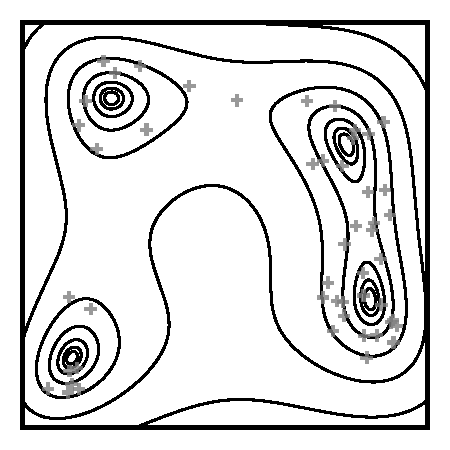
\includegraphics[width=\textwidth]{figures/himmelblau_samples.pdf}
        \end{center}
    \end{columns}
\end{frame}

% --- SLIDE 5: MCMC Sampling (4 minutes) ---
\begin{frame}<1-9>
    \frametitle{The Classic Workhorse: Markov Chain Monte Carlo (MCMC)}
    \begin{columns}[T]
        \column{0.5\textwidth}
        \only<1-5>{
        \begin{block}{How it Works (Metropolis-Hastings)}
            Imagine a ``walker'' exploring the parameter landscape.
            \begin{enumerate}
                \item Take a random step to a new position.
                \item If the new spot is ``higher'' (better likelihood), move there.
                \item If it's ``lower'', maybe move there anyway (with probability proportional to how much lower it is).
                \item Repeat millions of times. The path the walker takes traces the posterior distribution.
            \end{enumerate}
        \end{block}
        }
        \only<6-9>{
            \vspace{-1em}
        \begin{block}{Advantages \& Limitations}
            \begin{itemize}
                \item Explores the full posterior and gives uncertainties.
                \item \textcolor{red}{Limitation:} The walker can be inefficient. It can get ``stuck'' in a local high-likelihood region and fail to find other, separate modes.
                \item \textcolor{red}{Limitation:} Can be slow to explore highly correlated (``banana-shaped'') posteriors.
            \end{itemize}
        \end{block}
        \begin{alertblock}{Key Message}
            MCMC is a foundational sampling method, but its simple ``random walk'' can be inefficient in the complex parameter spaces of SED fitting.
        \end{alertblock}
        }
        \column{0.5\textwidth}
        \vspace{-1.8em}
        \begin{center}
            \includegraphics<1>[page=1]{figures/himmelblau_mcmc.pdf}%
            \includegraphics<2>[page=2]{figures/himmelblau_mcmc.pdf}%
            \includegraphics<3>[page=3]{figures/himmelblau_mcmc.pdf}%
            \includegraphics<4>[page=4]{figures/himmelblau_mcmc.pdf}%
            \includegraphics<5>[page=5]{figures/himmelblau_mcmc.pdf}%
            \includegraphics<6>[page=6]{figures/himmelblau_mcmc.pdf}%
            \includegraphics<7>[page=7]{figures/himmelblau_mcmc.pdf}%
            \includegraphics<8>[page=8]{figures/himmelblau_mcmc.pdf}%
            \includegraphics<9>[page=9]{figures/himmelblau_mcmc.pdf}%
        \end{center}
    \end{columns}
\end{frame}

% --- SLIDE 6: Ensemble Sampling (emcee) (4 minutes) ---
\begin{frame}<1-9>
    \frametitle{A Better Way: Ensemble Sampling (e.g., \texttt{emcee})}
    \begin{columns}[T]
        \column{0.5\textwidth}
        \only<1-5>{
        \begin{block}{How it Works}
            Instead of one walker, we use an \keyterm{ensemble} of hundreds of walkers.
            \begin{itemize}
                \item The walkers don't move completely randomly.
                \item They propose new steps based on the positions of \textit{other} walkers in the ensemble.
                \item This allows the whole group to learn about the shape of the posterior (e.g., its correlations) and explore it more efficiently.
            \end{itemize}
        \end{block}
        }
        \only<6-9>{
        \vspace{-1em}
        \begin{block}{Advantages}
            \begin{itemize}
                \item Much better at exploring correlated, ``banana-shaped'' parameter spaces.
                \item More efficient ``mixing'' than a single chain.
                \item Easy to parallelize (one walker per CPU).
            \end{itemize}
        \end{block}
        \begin{block}{Limitation}
            \begin{itemize}
                \item Ensemble can still get trapped in one mode if other modes are very far away.
            \end{itemize}
        \end{block}
        \begin{alertblock}{Key Message}
            Ensemble samplers like \texttt{emcee} are a major improvement for many problems, especially those with parameter degeneracies.
        \end{alertblock}
        }
        \column{0.5\textwidth}
        \vspace{-1.8em}
        \begin{center}
            \includegraphics<1>[width=\textwidth,page=1]{figures/himmelblau_emcee.pdf}%
            \includegraphics<2>[width=\textwidth,page=2]{figures/himmelblau_emcee.pdf}%
            \includegraphics<3>[width=\textwidth,page=3]{figures/himmelblau_emcee.pdf}%
            \includegraphics<4>[width=\textwidth,page=4]{figures/himmelblau_emcee.pdf}%
            \includegraphics<5>[width=\textwidth,page=5]{figures/himmelblau_emcee.pdf}%
            \includegraphics<6>[width=\textwidth,page=6]{figures/himmelblau_emcee.pdf}%
            \includegraphics<7>[width=\textwidth,page=7]{figures/himmelblau_emcee.pdf}%
            \includegraphics<8>[width=\textwidth,page=8]{figures/himmelblau_emcee.pdf}%
            \includegraphics<9>[width=\textwidth,page=9]{figures/himmelblau_emcee.pdf}%
        \end{center}
    \end{columns}
\end{frame}

% --- SLIDE 7: Nested Sampling (5 minutes) ---
\begin{frame}<1-8>
    \frametitle{The State of the Art: Nested Sampling (e.g., \texttt{dynesty})}
    \begin{columns}[T]
        \column{0.5\textwidth}
        \only<1-4>{
        \begin{block}{A Radically Different Approach}
            Instead of random walking, nested sampling attacks the problem from the outside-in.
            \begin{enumerate}
                \item Start with a set of ``live points'' scattered across the entire \keyterm{prior}.
                \item At each step: find the point with the \textit{worst} likelihood and discard it.
                \item Replace it with a new point drawn from the prior, but with a likelihood \textit{better} than the point you just discarded.
                \item This forces the set of live points to continuously ``shrink'' into regions of higher and higher likelihood.
            \end{enumerate}
        \end{block}
        }
        \only<5-8>{
        \begin{block}{Key Advantages}
            \begin{itemize}
                \item Naturally handles \keyterm{multimodality}. The shrinking cloud of points will find and explore all modes simultaneously.
                \item It calculates the \keyterm{Bayesian Evidence} ($\C[3]{\mathcal{Z}}$) as a primary output. This is essential for model comparison!
            \end{itemize}
        \end{block}
        \begin{alertblock}{Key Message}
            Nested sampling excels at exploring complex, multimodal posteriors and is the go-to method for Bayesian model comparison.
        \end{alertblock}
        }
        \column{0.5\textwidth}
        \vspace{-1.8em}
        \begin{center}
            \includegraphics<1>[width=\textwidth,page=1]{figures/himmelblau_ns.pdf}%
            \includegraphics<2>[width=\textwidth,page=2]{figures/himmelblau_ns.pdf}%
            \includegraphics<3>[width=\textwidth,page=3]{figures/himmelblau_ns.pdf}%
            \includegraphics<4>[width=\textwidth,page=4]{figures/himmelblau_ns.pdf}%
            \includegraphics<5>[width=\textwidth,page=5]{figures/himmelblau_ns.pdf}%
            \includegraphics<6>[width=\textwidth,page=6]{figures/himmelblau_ns.pdf}%
            \includegraphics<7>[width=\textwidth,page=7]{figures/himmelblau_ns.pdf}%
            \includegraphics<8>[width=\textwidth,page=8]{figures/himmelblau_ns.pdf}%
        \end{center}
    \end{columns}
\end{frame}

% --- SLIDE 8: How Nested Sampling Estimates Volumes (2 minutes) ---
\begin{frame}<1-9>
    \frametitle{How Nested Sampling Estimates Volumes: The Counting Trick}
    \begin{columns}[T]
        \column{0.5\textwidth}
        \begin{block}{Volume Contraction}
            At each step, the volume contracts predictably:
            \[V_{i+1} = V_i \times \frac{n_{\text{inside}}}{n_{\text{total}}}\]
            indep.\ of dimensionality, geometry or topology
        \end{block}
        
        \begin{columns}[T]
            \column{0.45\textwidth}
            \begin{block}{Evidence}
                The evidence is computed as:
                \[\mathcal{Z} = \sum \mathcal{L}_i \Delta V_i\]
            \end{block}
            
            \column{0.45\textwidth}
            \begin{block}{Posterior}
                Each sample gets importance weight:
                \[w_i = \mathcal{L}_i \times \Delta V_i\]
            \end{block}
        \end{columns}
        \column{0.5\textwidth}
        \vspace{-1.8em}
        \begin{center}
            \includegraphics<1>[width=\textwidth,page=1]{figures/himmelblau_ns_counting_trick.pdf}
            \includegraphics<2>[width=\textwidth,page=2]{figures/himmelblau_ns_counting_trick.pdf}
            \includegraphics<3>[width=\textwidth,page=3]{figures/himmelblau_ns_counting_trick.pdf}
            \includegraphics<4>[width=\textwidth,page=4]{figures/himmelblau_ns_counting_trick.pdf}
            \includegraphics<5>[width=\textwidth,page=5]{figures/himmelblau_ns_counting_trick.pdf}
            \includegraphics<6>[width=\textwidth,page=6]{figures/himmelblau_ns_counting_trick.pdf}
            \includegraphics<7>[width=\textwidth,page=7]{figures/himmelblau_ns_counting_trick.pdf}
            \includegraphics<8>[width=\textwidth,page=8]{figures/himmelblau_ns_counting_trick.pdf}
            \includegraphics<9>[width=\textwidth,page=9]{figures/himmelblau_ns_counting_trick.pdf}
        \end{center}
        \begin{center}
            \only<1>{\textbf{200 live points}}
            \only<2>{\textbf{Mark for deletion}}
            \only<3>{\textbf{Delete points}}
            \only<4>{\textbf{Repopulate}}
            \only<5>{\textbf{Next iteration}}
            \only<6>{\textbf{Delete again}}
            \only<7>{\textbf{Repopulate again}}
            \only<8>{\textbf{Complete sampling}}
            \only<9>{\textbf{Posterior reweighting}}
        \end{center}
    \end{columns}
\end{frame}

% --- SLIDE 9: Method Comparison (2 minutes) ---
\begin{frame}
    \frametitle{Choosing Your Tool: A Summary}
    \framesubtitle{No single best method, only the right tool for the job}
    \begin{center}
        \begin{tabular}{|l|c|c|c|c|}
            \hline
            \textbf{Method} & \textbf{Speed} & \textbf{Uncertainties?} & \textbf{Handles Multimodality?} & \textbf{Evidence?} \\
            \hline
            \textbf{Optimization} ($\chi^2$) & \textcolor{green!50!black}{Very Fast} & \textcolor{red}{No} & \textcolor{red}{No} & \textcolor{red}{No} \\
            \hline
            \textbf{MCMC} (\texttt{pymc} etc) & \textcolor{orange}{Medium} & \textcolor{green!50!black}{Yes} & \textcolor{orange}{Poorly} & \textcolor{red}{No} \\
            \hline
            \textbf{Ensemble} (\texttt{emcee}) & \textcolor{orange}{Medium} & \textcolor{green!50!black}{Yes} & \textcolor{orange}{Okay} & \textcolor{red}{No} \\
            \hline
            \textbf{Nested} (\texttt{dynesty}) & \textcolor{red}{Slower} & \textcolor{green!50!black}{Yes} & \textcolor{green!50!black}{Excellently} & \textcolor{green!50!black}{Yes!} \\
            \hline
        \end{tabular}
    \end{center}
    \begin{block}{Practical Guidance}
        \begin{itemize}
            \item \textbf{Quick exploration / Sanity check?} $\rightarrow$ Use Optimization.
            \item \textbf{Simple, well-behaved posterior?} $\rightarrow$ \texttt{emcee} is a great choice.
            \item \textbf{Complex, possibly multimodal posterior?} $\rightarrow$ Use \texttt{dynesty}.
            \item \textbf{Need to compare different physical models?} $\rightarrow$ You \textit{must} use Nested Sampling.
        \end{itemize}
    \end{block}
\end{frame}

% --- SLIDE 10: AI in Scientific Code Development (2 minutes) ---
\begin{frame}
    \frametitle{The Future: AI in Scientific Code Development}
    \framesubtitle{How these tools themselves are evolving}
    \vspace{-1em}
    \begin{columns}[T]
        \column{0.49\textwidth}
        \begin{block}{The Real AI Revolution: LLMs}
            The biggest impact of AI will not be in analyzing data, but in helping us write the code to do it.
            \begin{itemize}
                \item \keyterm{Automated code translation}: LLMs can help port legacy Fortran/C++ models to modern, GPU-friendly \& differentiable frameworks like JAX or PyTorch.
            \end{itemize}
        \end{block}
        \column{0.49\textwidth}
        \begin{block}{The 80/20 Rule of Scientific Work}
            \begin{itemize}
                \item \textbf{80\% ``boring'' tasks}: Writing code, debugging, drafting \& reviewing papers, munging data, organising meetings...
                \item \textbf{20\% ``hard thinking''}: The actual scientific insight.
            \end{itemize}
            AI's biggest immediate impact is automating and accelerating the 80\%, freeing up human time for the 20\%.
        \end{block}
    \end{columns}
    \begin{alertblock}{Key Message}
        AI is not just a tool for analysis; it's about to fundamentally change how we develop, optimize, and deploy our science
    \end{alertblock}
\end{frame}

% --- SLIDE 11: Conclusions (1 minute) ---
\begin{frame}
    \frametitle{Conclusions \& What's Next}
    \framesubtitle{\tthref{github.com/handley-lab/group}}
    \tikz[overlay,remember picture]
        \node[anchor=north east] (A) at ($(current page.north east)+(0,0)$) {
        
\includegraphics[width=0.06\textheight]{people/adam_ormondroyd.jpg}%
        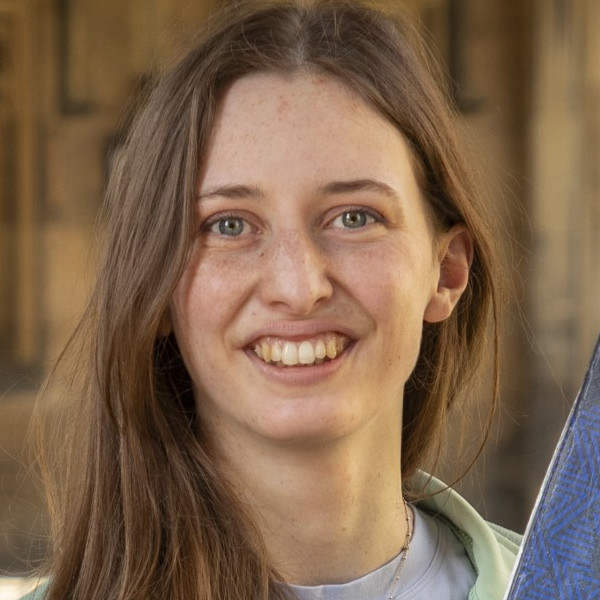
\includegraphics[width=0.06\textheight]{people/charlotte_priestley.jpg}%
        
\includegraphics[width=0.06\textheight]{people/claude.jpg}%
        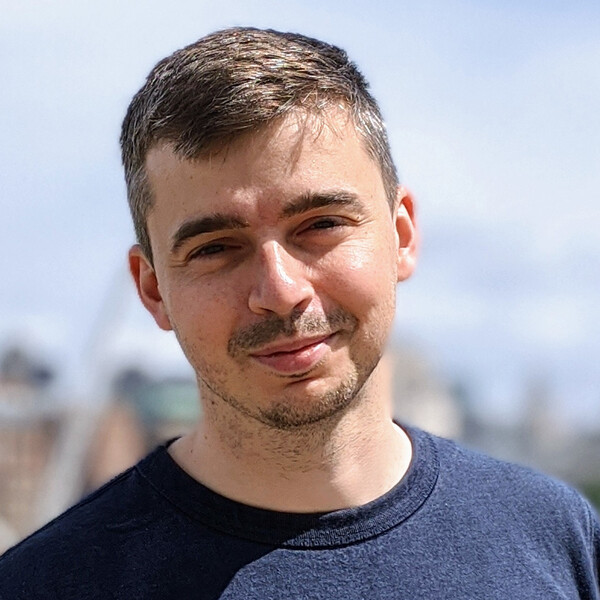
\includegraphics[width=0.06\textheight]{people/david_yallup.jpg}%
        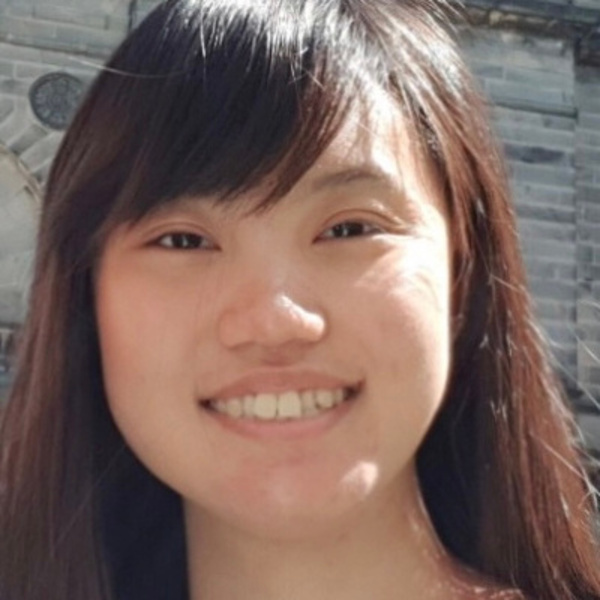
\includegraphics[width=0.06\textheight]{people/dily_ong.jpg}%
        
\includegraphics[width=0.06\textheight]{people/gemini.jpg}%
        
\includegraphics[width=0.06\textheight]{people/harry_bevins.jpg}%
        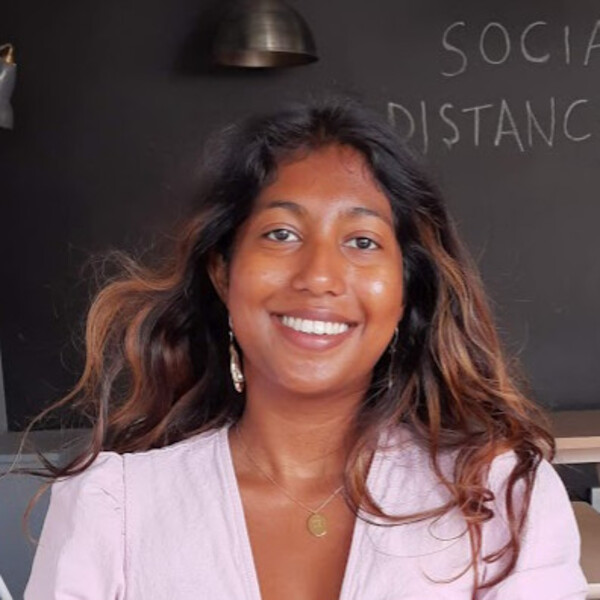
\includegraphics[width=0.06\textheight]{people/metha_prathaban.jpg}%
        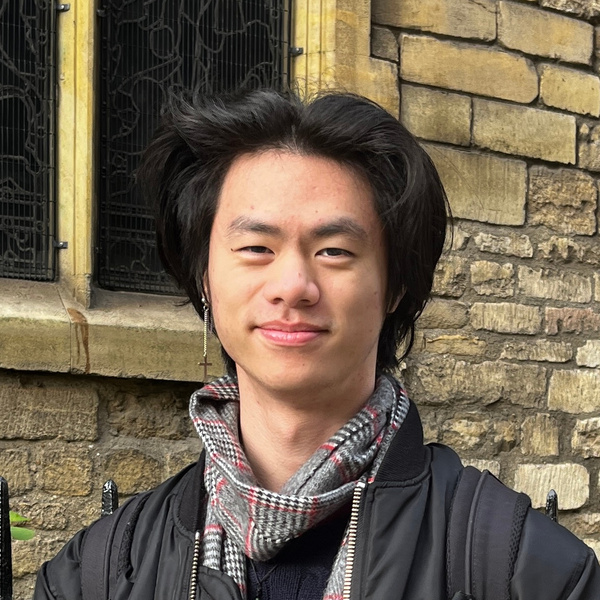
\includegraphics[width=0.06\textheight]{people/ming_yang.jpg}%
        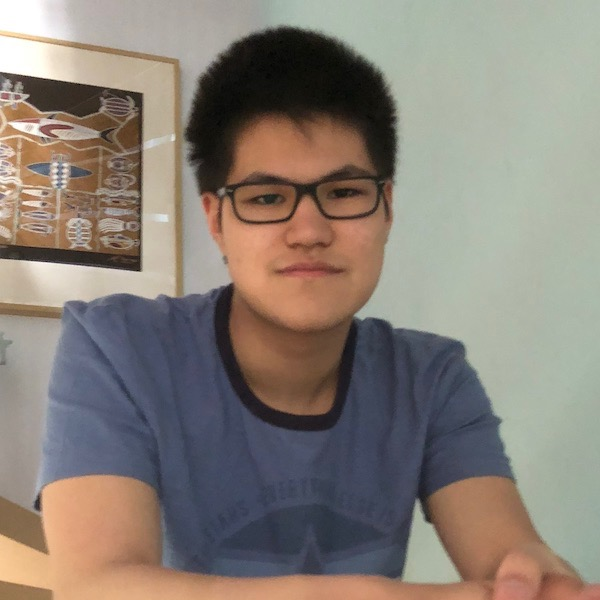
\includegraphics[width=0.06\textheight]{people/namu_kroupa.jpg}%
        
\includegraphics[width=0.06\textheight]{people/openai.jpg}%
        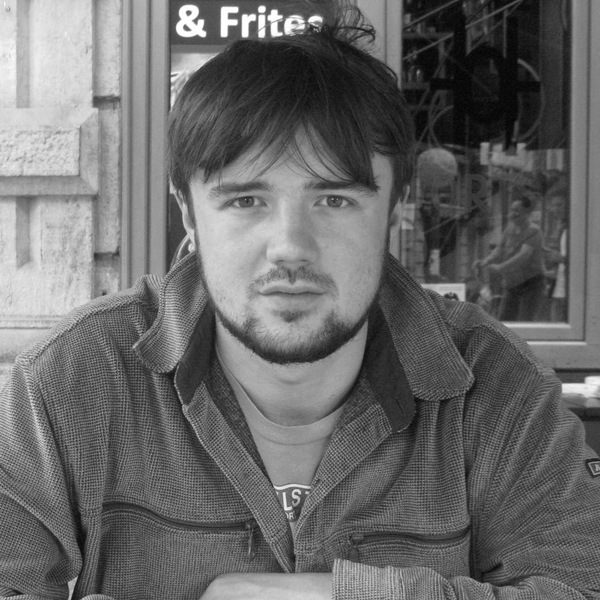
\includegraphics[width=0.06\textheight]{people/sam_leeney.jpg}%
        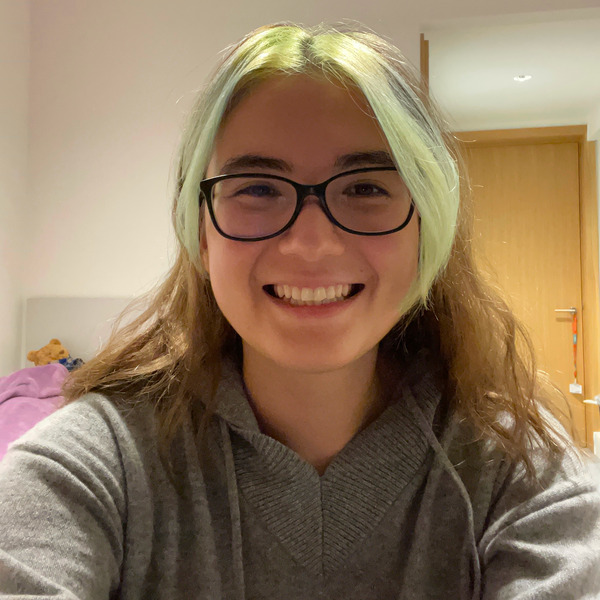
\includegraphics[width=0.06\textheight]{people/sinah_legner.jpg}%
        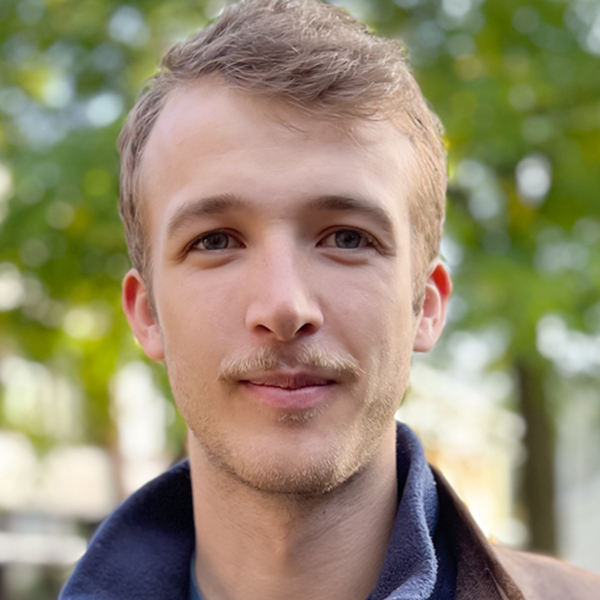
\includegraphics[width=0.06\textheight]{people/toby_lovick.jpg}%
        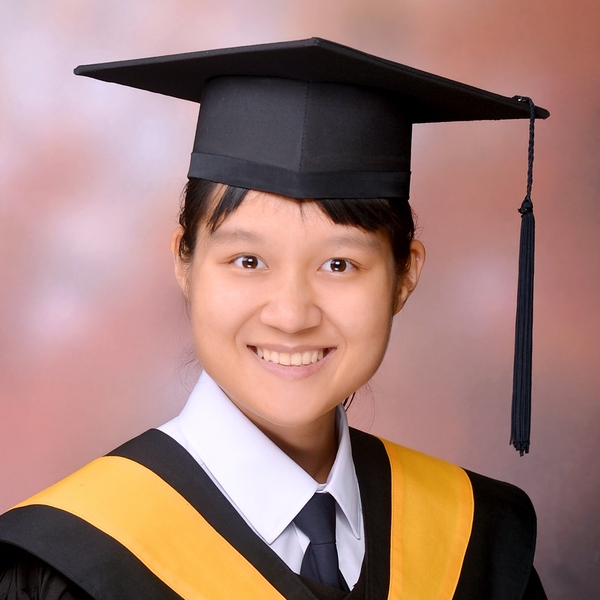
\includegraphics[width=0.06\textheight]{people/wei-ning_deng.jpg}%
        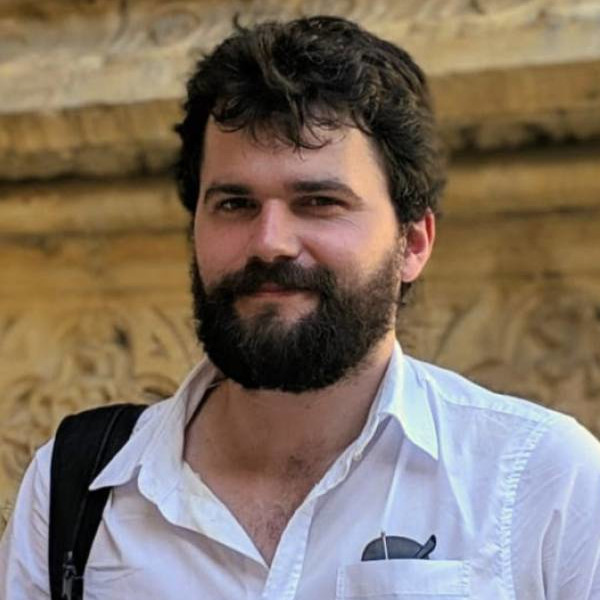
\includegraphics[width=0.06\textheight]{people/will_handley.jpg}%
        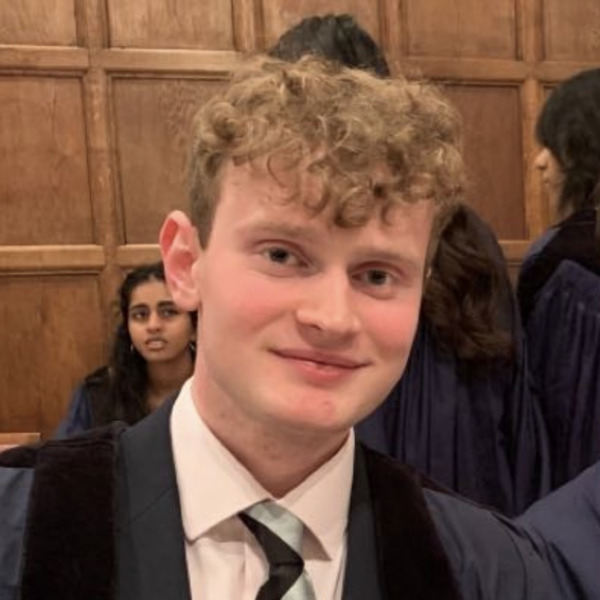
\includegraphics[width=0.06\textheight]{people/will_templeton.jpg}%
    };
    \begin{block}{Key Takeaways}
        \begin{itemize}
            \item SED fitting is a problem of \keyterm{statistical inference}, not just optimization.
            \item The goal is the full \keyterm{posterior distribution}, which gives us parameters \textit{and} their uncertainties.
            \item \keyterm{Sampling} methods are the tools we use to map out the posterior.
            \item The choice of sampler—from MCMC to Ensemble to Nested—depends on the complexity of your problem and whether you need to do \keyterm{model comparison}.
        \end{itemize}
    \end{block}
    \begin{alertblock}{Next Up: David Yallup on ``GPU Accelerated Nested Sampling''}
        Now that we know \textit{why} nested sampling is so powerful, we'll hear about how to make it \textit{fast}!
    \end{alertblock}
\end{frame}

% --- APPENDIX: HMC Sampling ---
\appendix

\begin{frame}<1-9>
    \frametitle{Appendix: Hamiltonian Monte Carlo (HMC)}
    \begin{columns}[T]
        \column{0.5\textwidth}
        \only<1-5>{
        \begin{block}{How it Works}
            Uses gradients to guide exploration more efficiently than random walks.
            \begin{enumerate}
                \item Treat parameters as ``particles'' with position and momentum.
                \item Use gradient of log-likelihood as ``force'' to guide movement.
                \item Propose coherent moves along gradient directions.
                \item Accept/reject using Metropolis criterion.
            \end{enumerate}
        \end{block}
        }
        \only<6-9>{
        \begin{block}{Advantages \& Requirements}
            \begin{itemize}
                \item Much more efficient than random walk for smooth posteriors.
                \item Requires gradients of the likelihood function.
                \item Can traverse parameter space much faster.
                \item Less likely to get stuck in local regions.
            \end{itemize}
        \end{block}
        \begin{alertblock}{Key Message}
            HMC leverages gradient information for efficient sampling, but requires differentiable models.
        \end{alertblock}
        }
        \column{0.5\textwidth}
        \vspace{-1.8em}
        \begin{center}
            \includegraphics<1>[width=\textwidth,page=1]{figures/himmelblau_hmc.pdf}%
            \includegraphics<2>[width=\textwidth,page=2]{figures/himmelblau_hmc.pdf}%
            \includegraphics<3>[width=\textwidth,page=3]{figures/himmelblau_hmc.pdf}%
            \includegraphics<4>[width=\textwidth,page=4]{figures/himmelblau_hmc.pdf}%
            \includegraphics<5>[width=\textwidth,page=5]{figures/himmelblau_hmc.pdf}%
            \includegraphics<6>[width=\textwidth,page=6]{figures/himmelblau_hmc.pdf}%
            \includegraphics<7>[width=\textwidth,page=7]{figures/himmelblau_hmc.pdf}%
            \includegraphics<8>[width=\textwidth,page=8]{figures/himmelblau_hmc.pdf}%
            \includegraphics<9>[width=\textwidth,page=9]{figures/himmelblau_hmc.pdf}%
        \end{center}
    \end{columns}
\end{frame}

\end{document}
